\chapter{树算法}

\index{tree}

\key{树}是由 $n$ 个节点和 $n-1$ 条边组成的连通无环图。从树中删除任意一条边都会把它分成两个连通分量，而向树中添加任意一条边都会形成环。此外，树中任意两个节点之间始终存在唯一一条路径。

例如，下图中的树包含 8 个节点和 7 条边：
\begin{center}
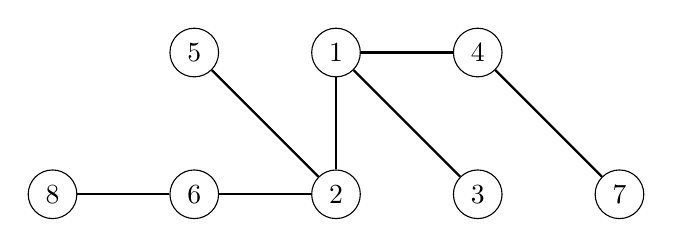
\begin{tikzpicture}[scale=0.9]
\node[draw, circle] (1) at (0,3) {$1$};
\node[draw, circle] (2) at (2,3) {$4$};
\node[draw, circle] (3) at (0,1) {$2$};
\node[draw, circle] (4) at (2,1) {$3$};
\node[draw, circle] (5) at (4,1) {$7$};
\node[draw, circle] (6) at (-2,3) {$5$};
\node[draw, circle] (7) at (-2,1) {$6$};
\node[draw, circle] (8) at (-4,1) {$8$};
\path[draw,thick,-] (1) -- (2);
\path[draw,thick,-] (1) -- (3);
\path[draw,thick,-] (1) -- (4);
\path[draw,thick,-] (2) -- (5);
\path[draw,thick,-] (3) -- (6);
\path[draw,thick,-] (3) -- (7);
\path[draw,thick,-] (7) -- (8);
\end{tikzpicture}
\end{center}

\index{leaf}

树的\key{叶节点}是度数为 1 的节点，也就是只有一个邻居的节点。例如，上述树的叶节点为 3、5、7 和 8。

\index{root}
\index{rooted tree}

在\key{有根树}中，选定一个节点作为树的\key{根}，其他节点都位于根的下方。例如，在下图中，节点 1 是根节点。

\begin{center}
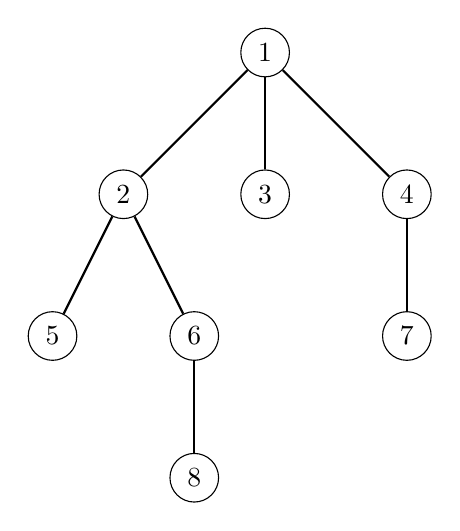
\begin{tikzpicture}[scale=0.9]
\node[draw, circle] (1) at (0,3) {$1$};
\node[draw, circle] (4) at (2,1) {$4$};
\node[draw, circle] (2) at (-2,1) {$2$};
\node[draw, circle] (3) at (0,1) {$3$};
\node[draw, circle] (7) at (2,-1) {$7$};
\node[draw, circle] (5) at (-3,-1) {$5$};
\node[draw, circle] (6) at (-1,-1) {$6$};
\node[draw, circle] (8) at (-1,-3) {$8$};
\path[draw,thick,-] (1) -- (2);
\path[draw,thick,-] (1) -- (3);
\path[draw,thick,-] (1) -- (4);
\path[draw,thick,-] (2) -- (5);
\path[draw,thick,-] (2) -- (6);
\path[draw,thick,-] (4) -- (7);
\path[draw,thick,-] (6) -- (8);
\end{tikzpicture}
\end{center}
\index{child}
\index{parent}

在有根树中，一个节点下方的邻居称为它的\key{子节点}，上方的邻居称为它的\key{父节点}。除没有父节点的根以外，每个节点恰有一个父节点。例如，在上图中，节点 2 的子节点是节点 5 和 6，它的父节点是节点 1。

\index{subtree}

有根树的结构是\emph{递归的}：树中每个节点都可以作为一棵\key{子树}的根，这棵子树包含该节点本身，以及其所有子节点的子树中的节点。例如，在上图中，节点 2 的子树由节点 2、5、6 和 8 构成：
\begin{center}
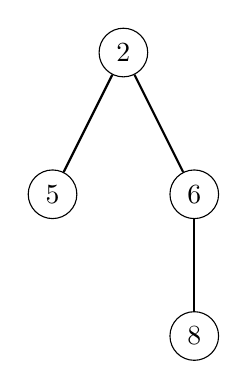
\begin{tikzpicture}[scale=0.9]
\node[draw, circle] (2) at (-2,1) {$2$};
\node[draw, circle] (5) at (-3,-1) {$5$};
\node[draw, circle] (6) at (-1,-1) {$6$};
\node[draw, circle] (8) at (-1,-3) {$8$};
\path[draw,thick,-] (2) -- (5);
\path[draw,thick,-] (2) -- (6);
\path[draw,thick,-] (6) -- (8);
\end{tikzpicture}
\end{center}

\section{树的遍历}

一般的图遍历算法也能用于遍历树的节点。不过，树的遍历比一般图的遍历更容易实现，因为树中没有环，也不可能从多个方向到达同一个节点。

遍历树的典型方法是从任意节点开始深度优先搜索。可以使用以下递归函数：

\begin{lstlisting}
void dfs(int s, int e) {
    // process node s
    for (auto u : adj[s]) {
        if (u != e) dfs(u, s);
    }
}
\end{lstlisting}

函数接收两个参数：当前节点 $s$ 和前一个节点 $e$。参数 $e$ 用来保证搜索只移动到尚未访问的节点。

下面的函数调用从节点 $x$ 开始搜索：

\begin{lstlisting}
dfs(x, 0);
\end{lstlisting}

第一次调用时 $e=0$，因为没有前一个节点，可以沿树中的任意方向前进。

\subsubsection{动态规划}

可以在树的遍历过程中使用动态规划计算某些信息。例如，利用动态规划，可以在 $O(n)$ 时间内为有根树中的每个节点计算其子树的节点数，或者从该节点到叶节点的最长路径长度。

例如，为每个节点 $s$ 计算值 $\texttt{count}[s]$，即其子树中的节点数。子树包含节点本身以及其各个子节点的子树中的所有节点，因此可以用以下代码递归计算节点数：

\begin{lstlisting}
void dfs(int s, int e) {
    count[s] = 1;
    for (auto u : adj[s]) {
        if (u == e) continue;
        dfs(u, s);
        count[s] += count[u];
    }
}
\end{lstlisting}

\section{直径}

\index{diameter}

树的\key{直径}是任意两个节点之间路径长度的最大值。例如，考虑下图：
\begin{center}
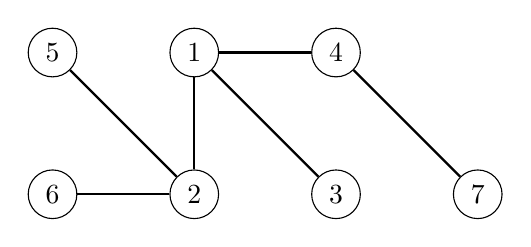
\begin{tikzpicture}[scale=0.9]
\node[draw, circle] (1) at (0,3) {$1$};
\node[draw, circle] (2) at (2,3) {$4$};
\node[draw, circle] (3) at (0,1) {$2$};
\node[draw, circle] (4) at (2,1) {$3$};
\node[draw, circle] (5) at (4,1) {$7$};
\node[draw, circle] (6) at (-2,3) {$5$};
\node[draw, circle] (7) at (-2,1) {$6$};
\path[draw,thick,-] (1) -- (2);
\path[draw,thick,-] (1) -- (3);
\path[draw,thick,-] (1) -- (4);
\path[draw,thick,-] (2) -- (5);
\path[draw,thick,-] (3) -- (6);
\path[draw,thick,-] (3) -- (7);
\end{tikzpicture}
\end{center}
这棵树的直径为 4，对应下列路径：
\begin{center}
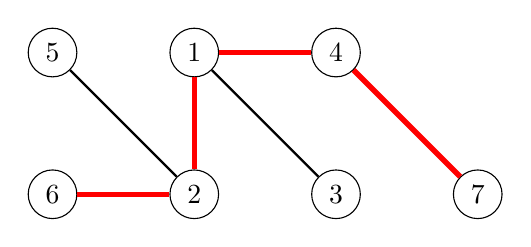
\begin{tikzpicture}[scale=0.9]
\node[draw, circle] (1) at (0,3) {$1$};
\node[draw, circle] (2) at (2,3) {$4$};
\node[draw, circle] (3) at (0,1) {$2$};
\node[draw, circle] (4) at (2,1) {$3$};
\node[draw, circle] (5) at (4,1) {$7$};
\node[draw, circle] (6) at (-2,3) {$5$};
\node[draw, circle] (7) at (-2,1) {$6$};
\path[draw,thick,-] (1) -- (2);
\path[draw,thick,-] (1) -- (3);
\path[draw,thick,-] (1) -- (4);
\path[draw,thick,-] (2) -- (5);
\path[draw,thick,-] (3) -- (6);
\path[draw,thick,-] (3) -- (7);

\path[draw,thick,-,color=red,line width=2pt] (7) -- (3);
\path[draw,thick,-,color=red,line width=2pt] (3) -- (1);
\path[draw,thick,-,color=red,line width=2pt] (1) -- (2);
\path[draw,thick,-,color=red,line width=2pt] (2) -- (5);
\end{tikzpicture}
\end{center}
最长路径可能不止一条。在上面的路径中，可以把节点 6 换成节点 5，得到另一条长度为 4 的路径。

下面介绍两种在 $O(n)$ 时间内计算树直径的算法。第一种基于动态规划，第二种使用两次深度优先搜索。

\subsubsection{算法 1}

处理许多树上问题的一般方法，是先任意选根，再尝试分别解决每棵子树上的问题。第一种直径算法正是基于这一思想。

一个重要观察是，有根树中的每条路径都有一个\emph{最高点}，即路径上位置最高的节点。因此，可以为每个节点计算以它为最高点的最长路径。这样的路径中必有一条对应树的直径。

例如，在下图中，节点 1 是直径所对应路径的最高点：
\begin{center}
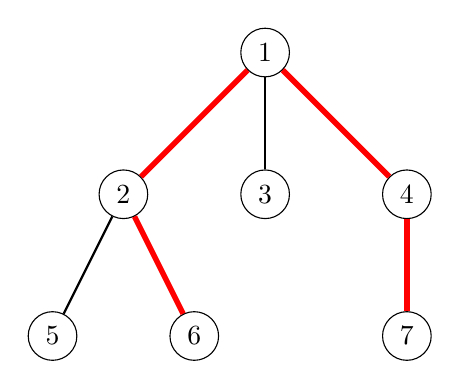
\begin{tikzpicture}[scale=0.9]
\node[draw, circle] (1) at (0,3) {$1$};
\node[draw, circle] (2) at (2,1) {$4$};
\node[draw, circle] (3) at (-2,1) {$2$};
\node[draw, circle] (4) at (0,1) {$3$};
\node[draw, circle] (5) at (2,-1) {$7$};
\node[draw, circle] (6) at (-3,-1) {$5$};
\node[draw, circle] (7) at (-1,-1) {$6$};
\path[draw,thick,-] (1) -- (2);
\path[draw,thick,-] (1) -- (3);
\path[draw,thick,-] (1) -- (4);
\path[draw,thick,-] (2) -- (5);
\path[draw,thick,-] (3) -- (6);
\path[draw,thick,-] (3) -- (7);

\path[draw,thick,-,color=red,line width=2pt] (7) -- (3);
\path[draw,thick,-,color=red,line width=2pt] (3) -- (1);
\path[draw,thick,-,color=red,line width=2pt] (1) -- (2);
\path[draw,thick,-,color=red,line width=2pt] (2) -- (5);
\end{tikzpicture}
\end{center}

对每个节点 $x$ 计算两个值：
\begin{itemize}
\item $\texttt{toLeaf}(x)$：从 $x$ 到任意叶节点的路径的最大长度；
\item $\texttt{maxLength}(x)$：以 $x$ 为最高点的路径的最大长度。
\end{itemize}
例如，在上图中，$\texttt{toLeaf}(1)=2$，因为存在路径 $1 \rightarrow 2 \rightarrow 6$；$\texttt{maxLength}(1)=4$，因为存在路径 $6 \rightarrow 2 \rightarrow 1 \rightarrow 4 \rightarrow 7$。在这里，$\texttt{maxLength}(1)$ 就等于直径。

利用动态规划，可以在 $O(n)$ 时间内计算所有节点的上述值。计算 $\texttt{toLeaf}(x)$ 时，遍历 $x$ 的子节点，选择 $\texttt{toLeaf}(c)$ 最大的子节点 $c$，并在该值上加一。计算 $\texttt{maxLength}(x)$ 时，选择两个不同的子节点 $a$ 和 $b$，使 $\texttt{toLeaf}(a)+\texttt{toLeaf}(b)$ 最大，再给这个和加二。

\subsubsection{算法 2}

另一种计算树直径的高效方法基于两次深度优先搜索。首先在树中任取节点 $a$，找到离 $a$ 最远的节点 $b$；然后找到离 $b$ 最远的节点 $c$。树的直径就是 $b$ 与 $c$ 之间的距离。

在下图中，$a$、$b$ 和 $c$ 可以取为：
\begin{center}
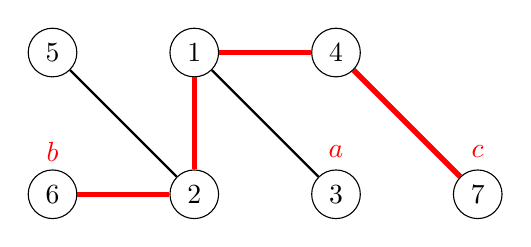
\begin{tikzpicture}[scale=0.9]
\node[draw, circle] (1) at (0,3) {$1$};
\node[draw, circle] (2) at (2,3) {$4$};
\node[draw, circle] (3) at (0,1) {$2$};
\node[draw, circle] (4) at (2,1) {$3$};
\node[draw, circle] (5) at (4,1) {$7$};
\node[draw, circle] (6) at (-2,3) {$5$};
\node[draw, circle] (7) at (-2,1) {$6$};
\path[draw,thick,-] (1) -- (2);
\path[draw,thick,-] (1) -- (3);
\path[draw,thick,-] (1) -- (4);
\path[draw,thick,-] (2) -- (5);
\path[draw,thick,-] (3) -- (6);
\path[draw,thick,-] (3) -- (7);
\node[color=red] at (2,1.6) {$a$};
\node[color=red] at (-2,1.6) {$b$};
\node[color=red] at (4,1.6) {$c$};

\path[draw,thick,-,color=red,line width=2pt] (7) -- (3);
\path[draw,thick,-,color=red,line width=2pt] (3) -- (1);
\path[draw,thick,-,color=red,line width=2pt] (1) -- (2);
\path[draw,thick,-,color=red,line width=2pt] (2) -- (5);
\end{tikzpicture}
\end{center}

这个方法很巧妙，但它为什么正确？

把树换一种画法会更容易理解：让直径对应的路径水平放置，其他所有节点都悬挂在这条路径上：
\begin{center}
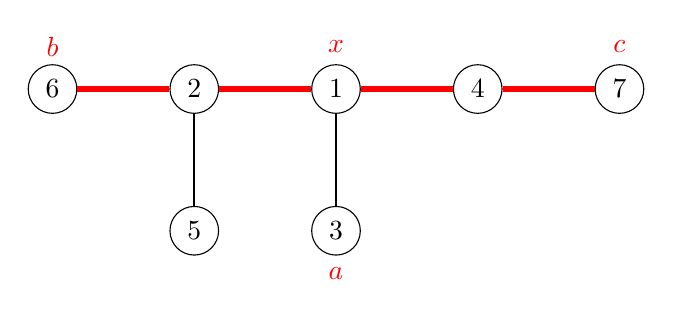
\begin{tikzpicture}[scale=0.9]
\node[draw, circle] (1) at (2,1) {$1$};
\node[draw, circle] (2) at (4,1) {$4$};
\node[draw, circle] (3) at (0,1) {$2$};
\node[draw, circle] (4) at (2,-1) {$3$};
\node[draw, circle] (5) at (6,1) {$7$};
\node[draw, circle] (6) at (0,-1) {$5$};
\node[draw, circle] (7) at (-2,1) {$6$};
\path[draw,thick,-] (1) -- (2);
\path[draw,thick,-] (1) -- (3);
\path[draw,thick,-] (1) -- (4);
\path[draw,thick,-] (2) -- (5);
\path[draw,thick,-] (3) -- (6);
\path[draw,thick,-] (3) -- (7);
\node[color=red] at (2,-1.6) {$a$};
\node[color=red] at (-2,1.6) {$b$};
\node[color=red] at (6,1.6) {$c$};
\node[color=red] at (2,1.6) {$x$};

\path[draw,thick,-,color=red,line width=2pt] (7) -- (3);
\path[draw,thick,-,color=red,line width=2pt] (3) -- (1);
\path[draw,thick,-,color=red,line width=2pt] (1) -- (2);
\path[draw,thick,-,color=red,line width=2pt] (2) -- (5);
\end{tikzpicture}
\end{center}

节点 $x$ 表示从节点 $a$ 出发的路径与直径路径汇合的位置。离 $a$ 最远的节点要么是 $b$，要么是 $c$，要么是某个与节点 $x$ 的距离至少同样远的其他节点。因此，这个节点总能作为某条直径路径的一个端点。

\section{所有最长路径}

下一个问题是：对树中的每个节点，计算从该节点出发的路径的最大长度。它可以看作树直径问题的推广，因为这些长度中的最大值就是树的直径。这个问题同样可以在 $O(n)$ 时间内解决。

例如，考虑下图：
\begin{center}
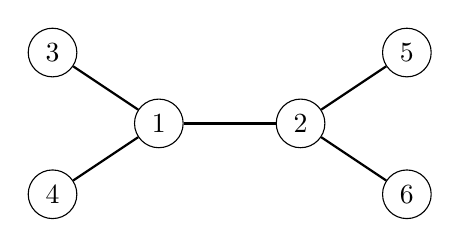
\begin{tikzpicture}[scale=0.9]
\node[draw, circle] (1) at (0,0) {$1$};
\node[draw, circle] (2) at (-1.5,-1) {$4$};
\node[draw, circle] (3) at (2,0) {$2$};
\node[draw, circle] (4) at (-1.5,1) {$3$};
\node[draw, circle] (6) at (3.5,-1) {$6$};
\node[draw, circle] (7) at (3.5,1) {$5$};
\path[draw,thick,-] (1) -- (2);
\path[draw,thick,-] (1) -- (3);
\path[draw,thick,-] (1) -- (4);
\path[draw,thick,-] (3) -- (6);
\path[draw,thick,-] (3) -- (7);
\end{tikzpicture}
\end{center}

令 $\texttt{maxLength}(x)$ 表示从节点 $x$ 出发的路径的最大长度。例如，在上图中，$\texttt{maxLength}(4)=3$，因为存在路径 $4 \rightarrow 1 \rightarrow 2 \rightarrow 6$。所有值如下表所示：
\begin{center}
\begin{tabular}{l|lllllll}
节点 $x$ & 1 & 2 & 3 & 4 & 5 & 6 \\
$\texttt{maxLength}(x)$ & 2 & 2 & 3 & 3 & 3 & 3 \\
\end{tabular}
\end{center}

同样，解决这个问题的良好起点是任意选定树根：
\begin{center}
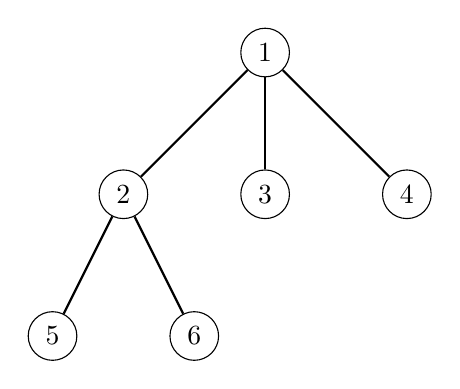
\begin{tikzpicture}[scale=0.9]
\node[draw, circle] (1) at (0,3) {$1$};
\node[draw, circle] (2) at (2,1) {$4$};
\node[draw, circle] (3) at (-2,1) {$2$};
\node[draw, circle] (4) at (0,1) {$3$};
\node[draw, circle] (6) at (-3,-1) {$5$};
\node[draw, circle] (7) at (-1,-1) {$6$};
\path[draw,thick,-] (1) -- (2);
\path[draw,thick,-] (1) -- (3);
\path[draw,thick,-] (1) -- (4);
\path[draw,thick,-] (3) -- (6);
\path[draw,thick,-] (3) -- (7);
\end{tikzpicture}
\end{center}

问题的第一部分是：对每个节点 $x$，计算经过 $x$ 的某个子节点的路径的最大长度。例如，从节点 1 出发的最长路径经过其子节点 2：
\begin{center}
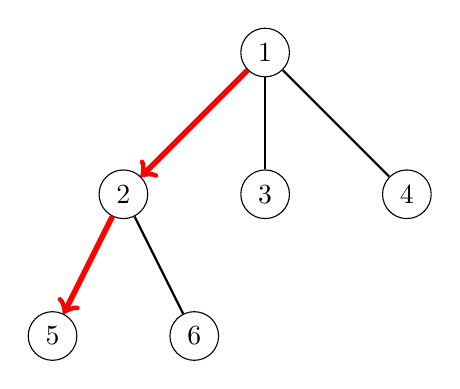
\begin{tikzpicture}[scale=0.9]
\node[draw, circle] (1) at (0,3) {$1$};
\node[draw, circle] (2) at (2,1) {$4$};
\node[draw, circle] (3) at (-2,1) {$2$};
\node[draw, circle] (4) at (0,1) {$3$};
\node[draw, circle] (6) at (-3,-1) {$5$};
\node[draw, circle] (7) at (-1,-1) {$6$};
\path[draw,thick,-] (1) -- (2);
\path[draw,thick,-] (1) -- (3);
\path[draw,thick,-] (1) -- (4);
\path[draw,thick,-] (3) -- (6);
\path[draw,thick,-] (3) -- (7);

\path[draw,thick,->,color=red,line width=2pt] (1) -- (3);
\path[draw,thick,->,color=red,line width=2pt] (3) -- (6);
\end{tikzpicture}
\end{center}
这一部分很容易在 $O(n)$ 时间内解决，因为可以像前面一样使用动态规划。

问题的第二部分是：对每个节点 $x$，计算经过其父节点 $p$ 的路径的最大长度。例如，从节点 3 出发的最长路径经过其父节点 1：
\begin{center}
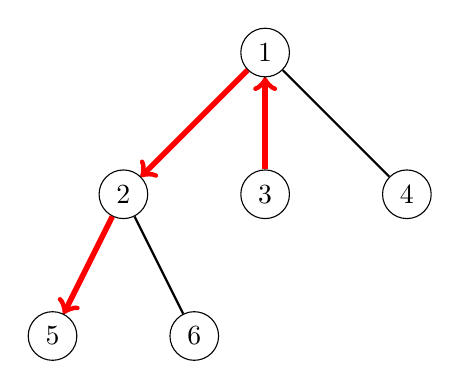
\begin{tikzpicture}[scale=0.9]
\node[draw, circle] (1) at (0,3) {$1$};
\node[draw, circle] (2) at (2,1) {$4$};
\node[draw, circle] (3) at (-2,1) {$2$};
\node[draw, circle] (4) at (0,1) {$3$};
\node[draw, circle] (6) at (-3,-1) {$5$};
\node[draw, circle] (7) at (-1,-1) {$6$};
\path[draw,thick,-] (1) -- (2);
\path[draw,thick,-] (1) -- (3);
\path[draw,thick,-] (1) -- (4);
\path[draw,thick,-] (3) -- (6);
\path[draw,thick,-] (3) -- (7);

\path[draw,thick,->,color=red,line width=2pt] (4) -- (1);
\path[draw,thick,->,color=red,line width=2pt] (1) -- (3);
\path[draw,thick,->,color=red,line width=2pt] (3) -- (6);
\end{tikzpicture}
\end{center}

乍看之下，似乎应选择从 $p$ 出发的最长路径。然而，这种做法\emph{并不}总是正确，因为从 $p$ 出发的最长路径可能经过 $x$。下面就是这种情形：
\begin{center}
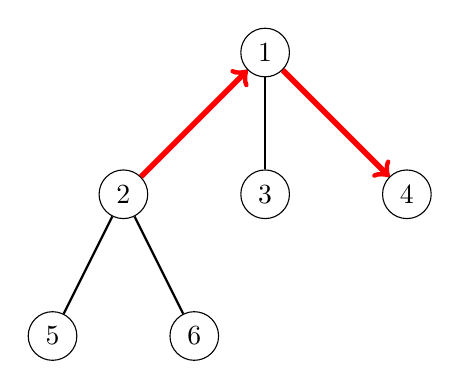
\begin{tikzpicture}[scale=0.9]
\node[draw, circle] (1) at (0,3) {$1$};
\node[draw, circle] (2) at (2,1) {$4$};
\node[draw, circle] (3) at (-2,1) {$2$};
\node[draw, circle] (4) at (0,1) {$3$};
\node[draw, circle] (6) at (-3,-1) {$5$};
\node[draw, circle] (7) at (-1,-1) {$6$};
\path[draw,thick,-] (1) -- (2);
\path[draw,thick,-] (1) -- (3);
\path[draw,thick,-] (1) -- (4);
\path[draw,thick,-] (3) -- (6);
\path[draw,thick,-] (3) -- (7);

\path[draw,thick,->,color=red,line width=2pt] (3) -- (1);
\path[draw,thick,->,color=red,line width=2pt] (1) -- (2);
\end{tikzpicture}
\end{center}

不过，只要为每个节点 $x$ 保存\emph{两个}最大长度，仍可在 $O(n)$ 时间内解决第二部分：
\begin{itemize}
\item $\texttt{maxLength}_1(x)$：从 $x$ 出发的路径的最大长度；
\item $\texttt{maxLength}_2(x)$：从 $x$ 出发、且方向不同于第一条路径的路径的最大长度。
\end{itemize}
例如，在上图中，沿路径 $1 \rightarrow 2 \rightarrow 5$ 可得 $\texttt{maxLength}_1(1)=2$，沿路径 $1 \rightarrow 3$ 可得 $\texttt{maxLength}_2(1)=1$。

最后，如果 $\texttt{maxLength}_1(p)$ 对应的路径经过 $x$，则最大长度为 $\texttt{maxLength}_2(p)+1$；否则为 $\texttt{maxLength}_1(p)+1$。

\section{二叉树}

\index{binary tree}

\begin{samepage}
\key{二叉树}是一种有根树，其中每个节点都有左子树和右子树。节点的某棵子树可以为空，因此二叉树中的每个节点有零个、一个或两个子节点。

例如，下图是一棵二叉树：
\begin{center}
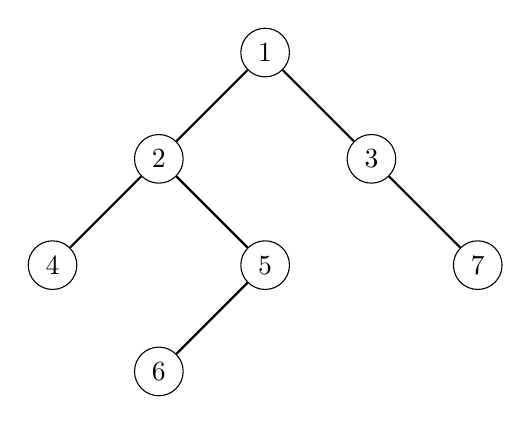
\begin{tikzpicture}[scale=0.9]
\node[draw, circle] (1) at (0,0) {$1$};
\node[draw, circle] (2) at (-1.5,-1.5) {$2$};
\node[draw, circle] (3) at (1.5,-1.5) {$3$};
\node[draw, circle] (4) at (-3,-3) {$4$};
\node[draw, circle] (5) at (0,-3) {$5$};
\node[draw, circle] (6) at (-1.5,-4.5) {$6$};
\node[draw, circle] (7) at (3,-3) {$7$};

\path[draw,thick,-] (1) -- (2);
\path[draw,thick,-] (1) -- (3);
\path[draw,thick,-] (2) -- (4);
\path[draw,thick,-] (2) -- (5);
\path[draw,thick,-] (5) -- (6);
\path[draw,thick,-] (3) -- (7);
\end{tikzpicture}
\end{center}
\end{samepage}

\index{pre-order}
\index{in-order}
\index{post-order}

二叉树的节点有三种自然顺序，分别对应递归遍历树的不同方式：

\begin{itemize}
\item \key{前序遍历}：先处理根，再遍历左子树，最后遍历右子树；
\item \key{中序遍历}：先遍历左子树，再处理根，最后遍历右子树；
\item \key{后序遍历}：先遍历左子树，再遍历右子树，最后处理根。
\end{itemize}

对上图中的树，前序遍历为 $[1,2,4,5,6,3,7]$，中序遍历为 $[4,2,6,5,1,3,7]$，后序遍历为 $[4,6,5,2,7,3,1]$。

若知道一棵树的前序和中序遍历，就能重建其准确结构。例如，上图是前序遍历为 $[1,2,4,5,6,3,7]$、中序遍历为 $[4,2,6,5,1,3,7]$ 的唯一一棵树。类似地，后序与中序遍历也能确定树的结构。

然而，如果只知道前序和后序遍历，情况就不同了：可能有多棵树符合这两个顺序。例如，在下面两棵树中，
\begin{center}
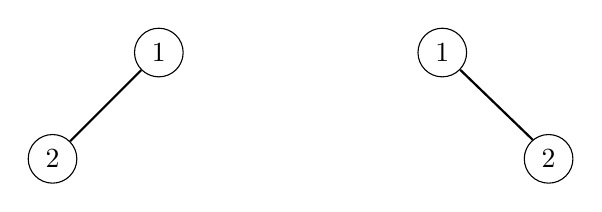
\begin{tikzpicture}[scale=0.9]
\node[draw, circle] (1) at (0,0) {$1$};
\node[draw, circle] (2) at (-1.5,-1.5) {$2$};
\path[draw,thick,-] (1) -- (2);

\node[draw, circle] (1b) at (0+4,0) {$1$};
\node[draw, circle] (2b) at (1.5+4,-1.5) {$2$};
\path[draw,thick,-] (1b) -- (2b);
\end{tikzpicture}
\end{center}
前序遍历都是 $[1,2]$，后序遍历都是 $[2,1]$，但树的结构不同。
